%%%%%%%%%%%%%%%%%%%%%%%%%%%%%%%%%%%%%%%%%%%%%%%%%%%%%%%%%%%%%%%%%%%%%%%%%%%%%%%
\section{Results}
\label{sec:results}
%%%%%%%%%%%%%%%%%%%%%%%%%%%%%%%%%%%%%%%%%%%%%%%%%%%%%%%%%%%%%%%%%%%%%%%%%%%%%%%

-motivate single-step approach
-describe infinite vs. null approaches
-describe simulation tools (i.e., OpenMOC)
-describe benchmarks
-present results




%%%%%%%%%%%%%%%%%%%%%%%%%%%%%%%%%%%%%%%%%%%%%
\subsection{Benchmarks and Reference Results}
\label{subsec:benchmarks}

This paper modeled benchmarks derived from the Benchmark for Evaluation And Validation of Reactor Simulations (BEAVRS) PWR model~\cite{horelik2013beavrs}. Each test case includes heterogeneous features -- and corresponding spatial self-shielding effects -- to demonstrate the potential utility of a single-step framework for MGXS generation. The benchmarks were comprised of materials from the BEAVRS model, including 1.6\% and 3.1\% enriched UO$_2$ fuel, borated water (975 ppm boron), zircaloy, helium, air, borosilicate glass and stainless steel. Each material was modeled with cross sections from the ENDF/B-VII.1 continuous energy cross section library~\cite{mcnpx2003manual} evaluated at 600K for hot zero power conditions. 

%Although BEAVRS is an axially heterogeneous 3D core model, both benchmarks were fabricated in 2D due to the geometric constraints in OpenMOC.

The first benchmark was a single fuel assembly with an array of 264 fuel pins of 1.6\% enriched UO$_2$ fuel with zircaloy cladding and a helium gap. The assembly included 24 control rod guide tubes (CRGTs) filled by borated water and surrounded by zircaloy cladding, and a central instrument tube filled with air surrounded by two zircaloy tubes separated by borated water. The second benchmark was constructed as a 2$\times$2 colorset of two fuel assemblies extracted from the BEAVRS model. The top-left and bottom-right fuel assemblies were of the same enrichment and configuration as the single assembly benchmark. The top-right and bottom-left fuel assemblies included 264 fuel pins of 3.1\% enriched UO$_2$ fuel, 20 CRGTs and a central instrument tube. In addition, the two 3.1\% enriched assemblies included four burnable poisons (BPs) consisting of eight layers of air, steel, borosilicate glass and zircaloy. The colorset was surrounded by a water reflector on the bottom and right that was of the same width as a fuel assembly. The assembly benchmark was modeled with reflective boundary conditions, while the colorset was modeled with reflective boundaries on the top and left and vacuum boundaries on the bottom and right. The assembly and colorset are illustrated in \autoref{fig:benchmarks-materials}.

%The intra-pin grid spacers and grid sleeves separating each assembly in the BEAVRS model were not included either benchmark. 

\begin{figure}[h!]
\centering
\begin{subfigure}{0.42\textwidth}
  \centering
  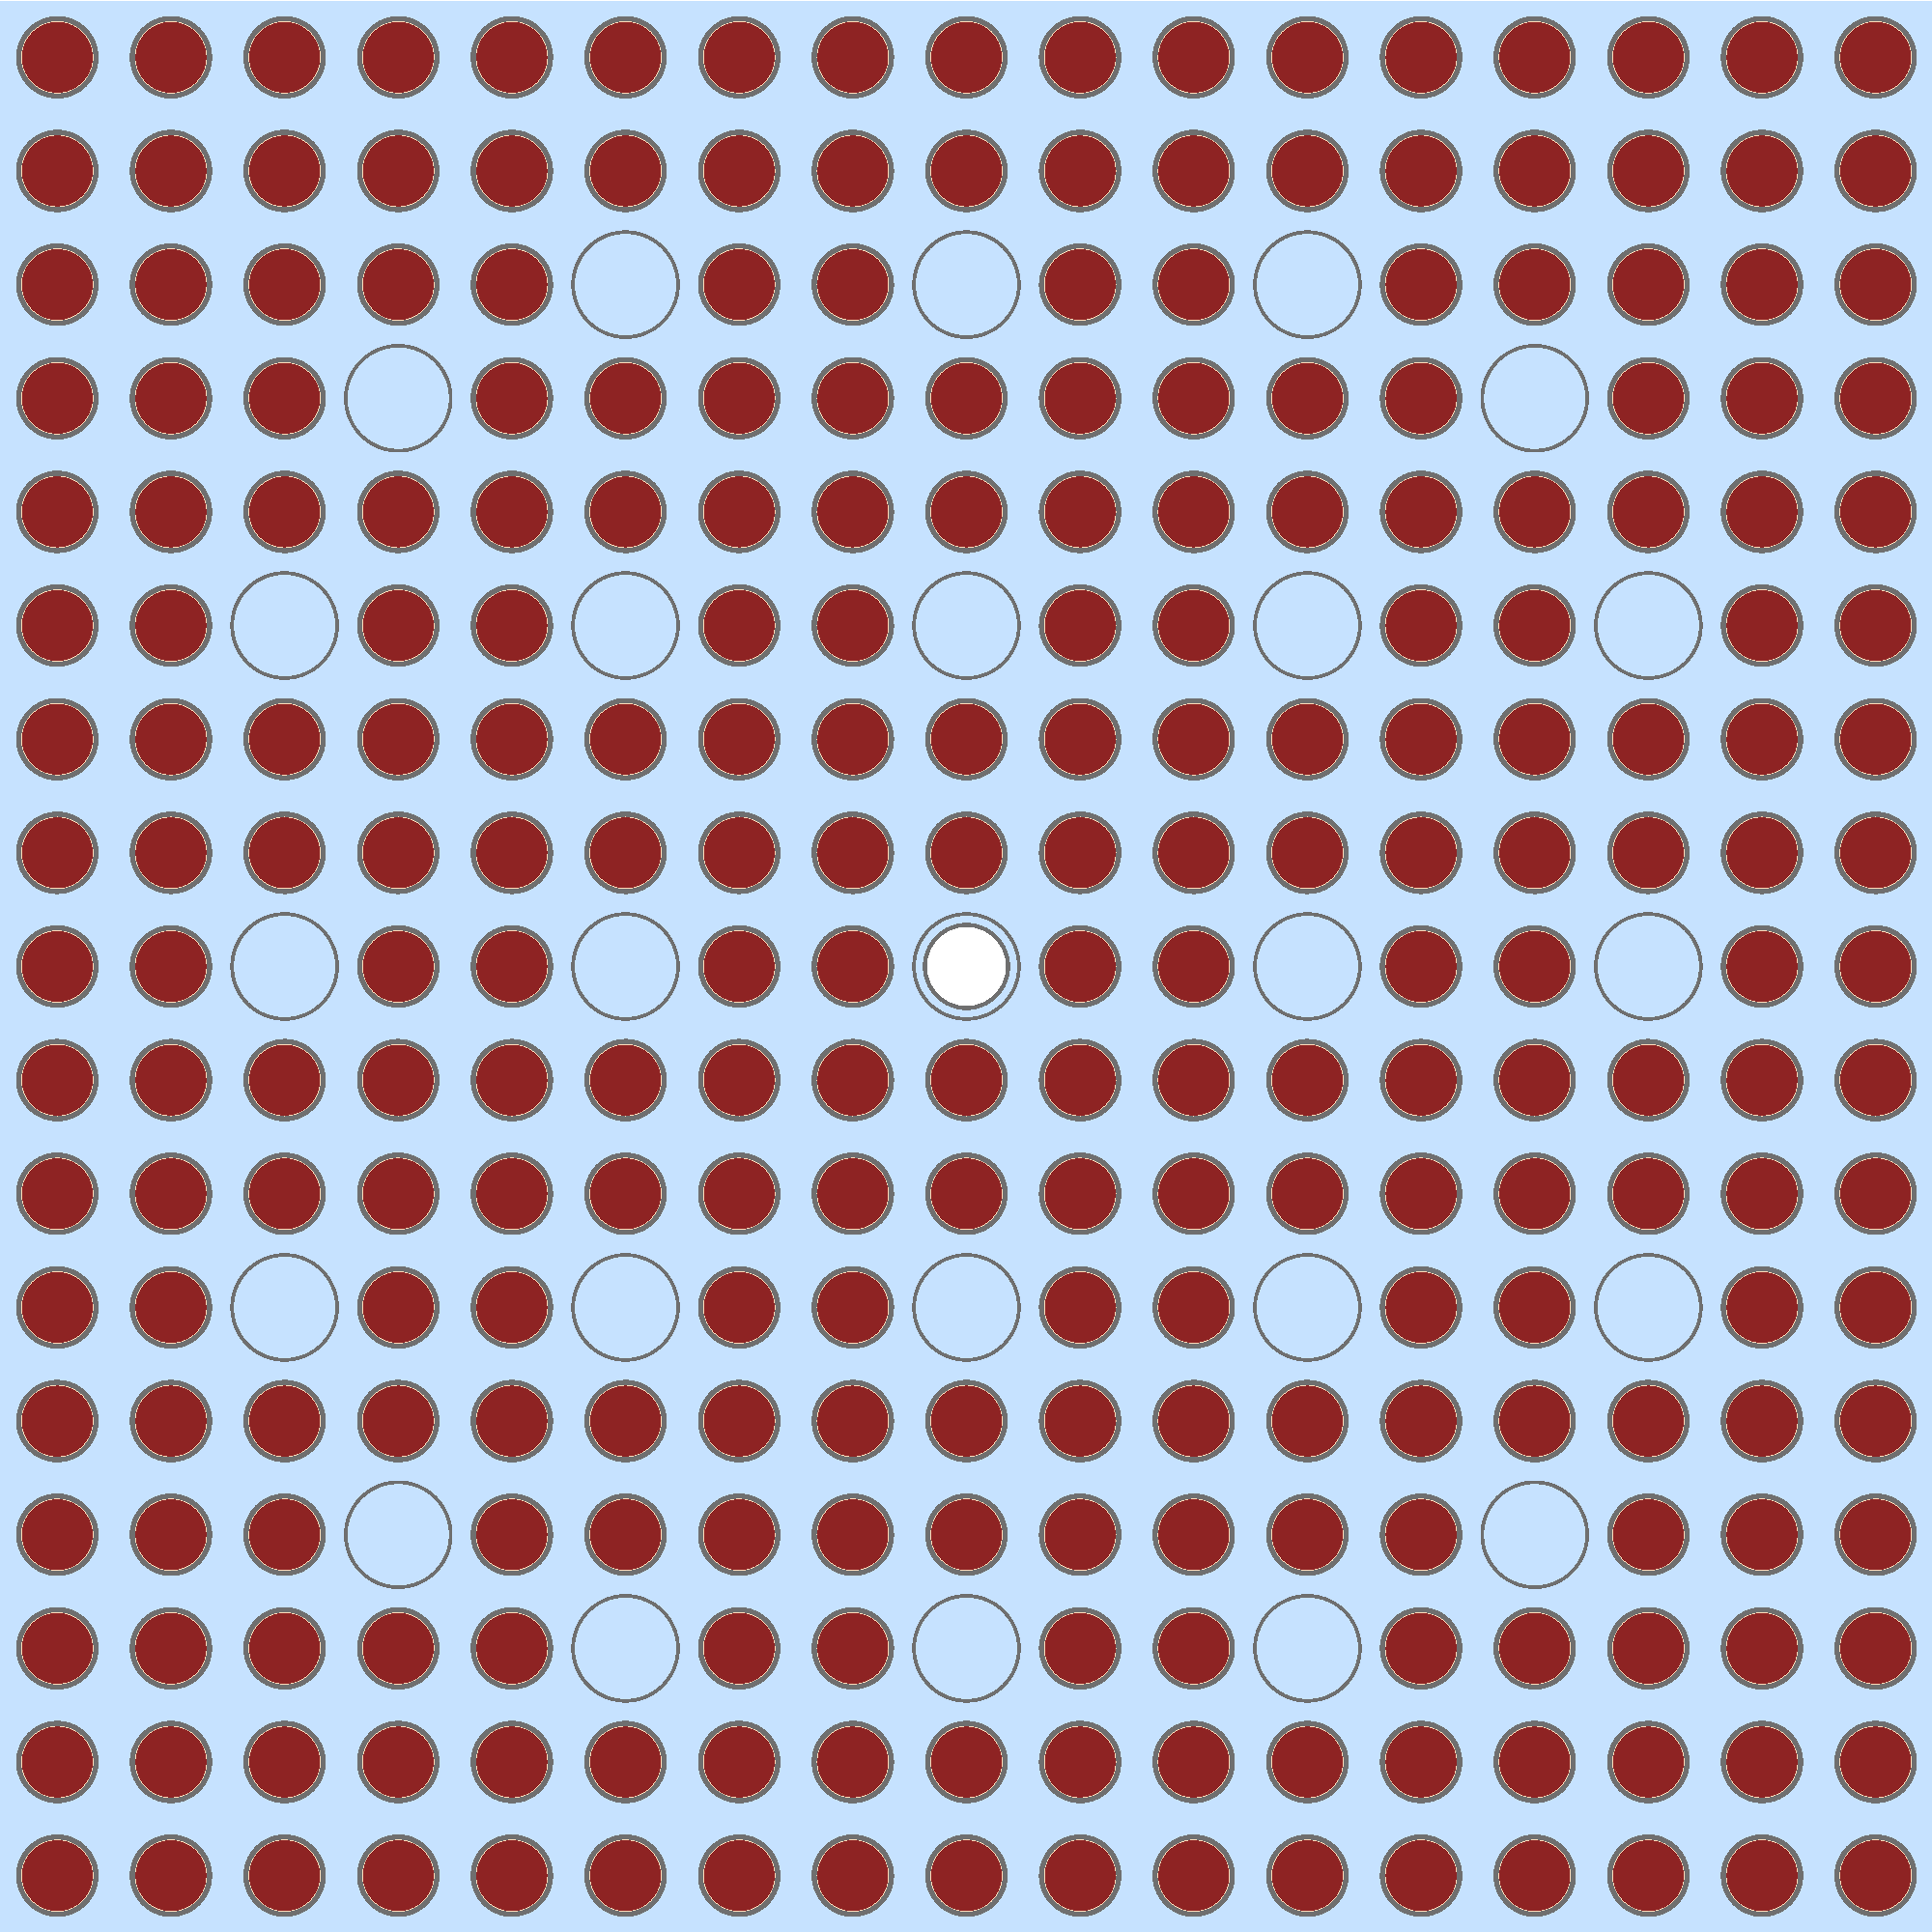
\includegraphics[width=0.8\linewidth]{figures/assembly/geometry}
  \caption{}
  \label{fig:benchmarks}
\end{subfigure}
\begin{subfigure}{0.42\textwidth}
  \centering
  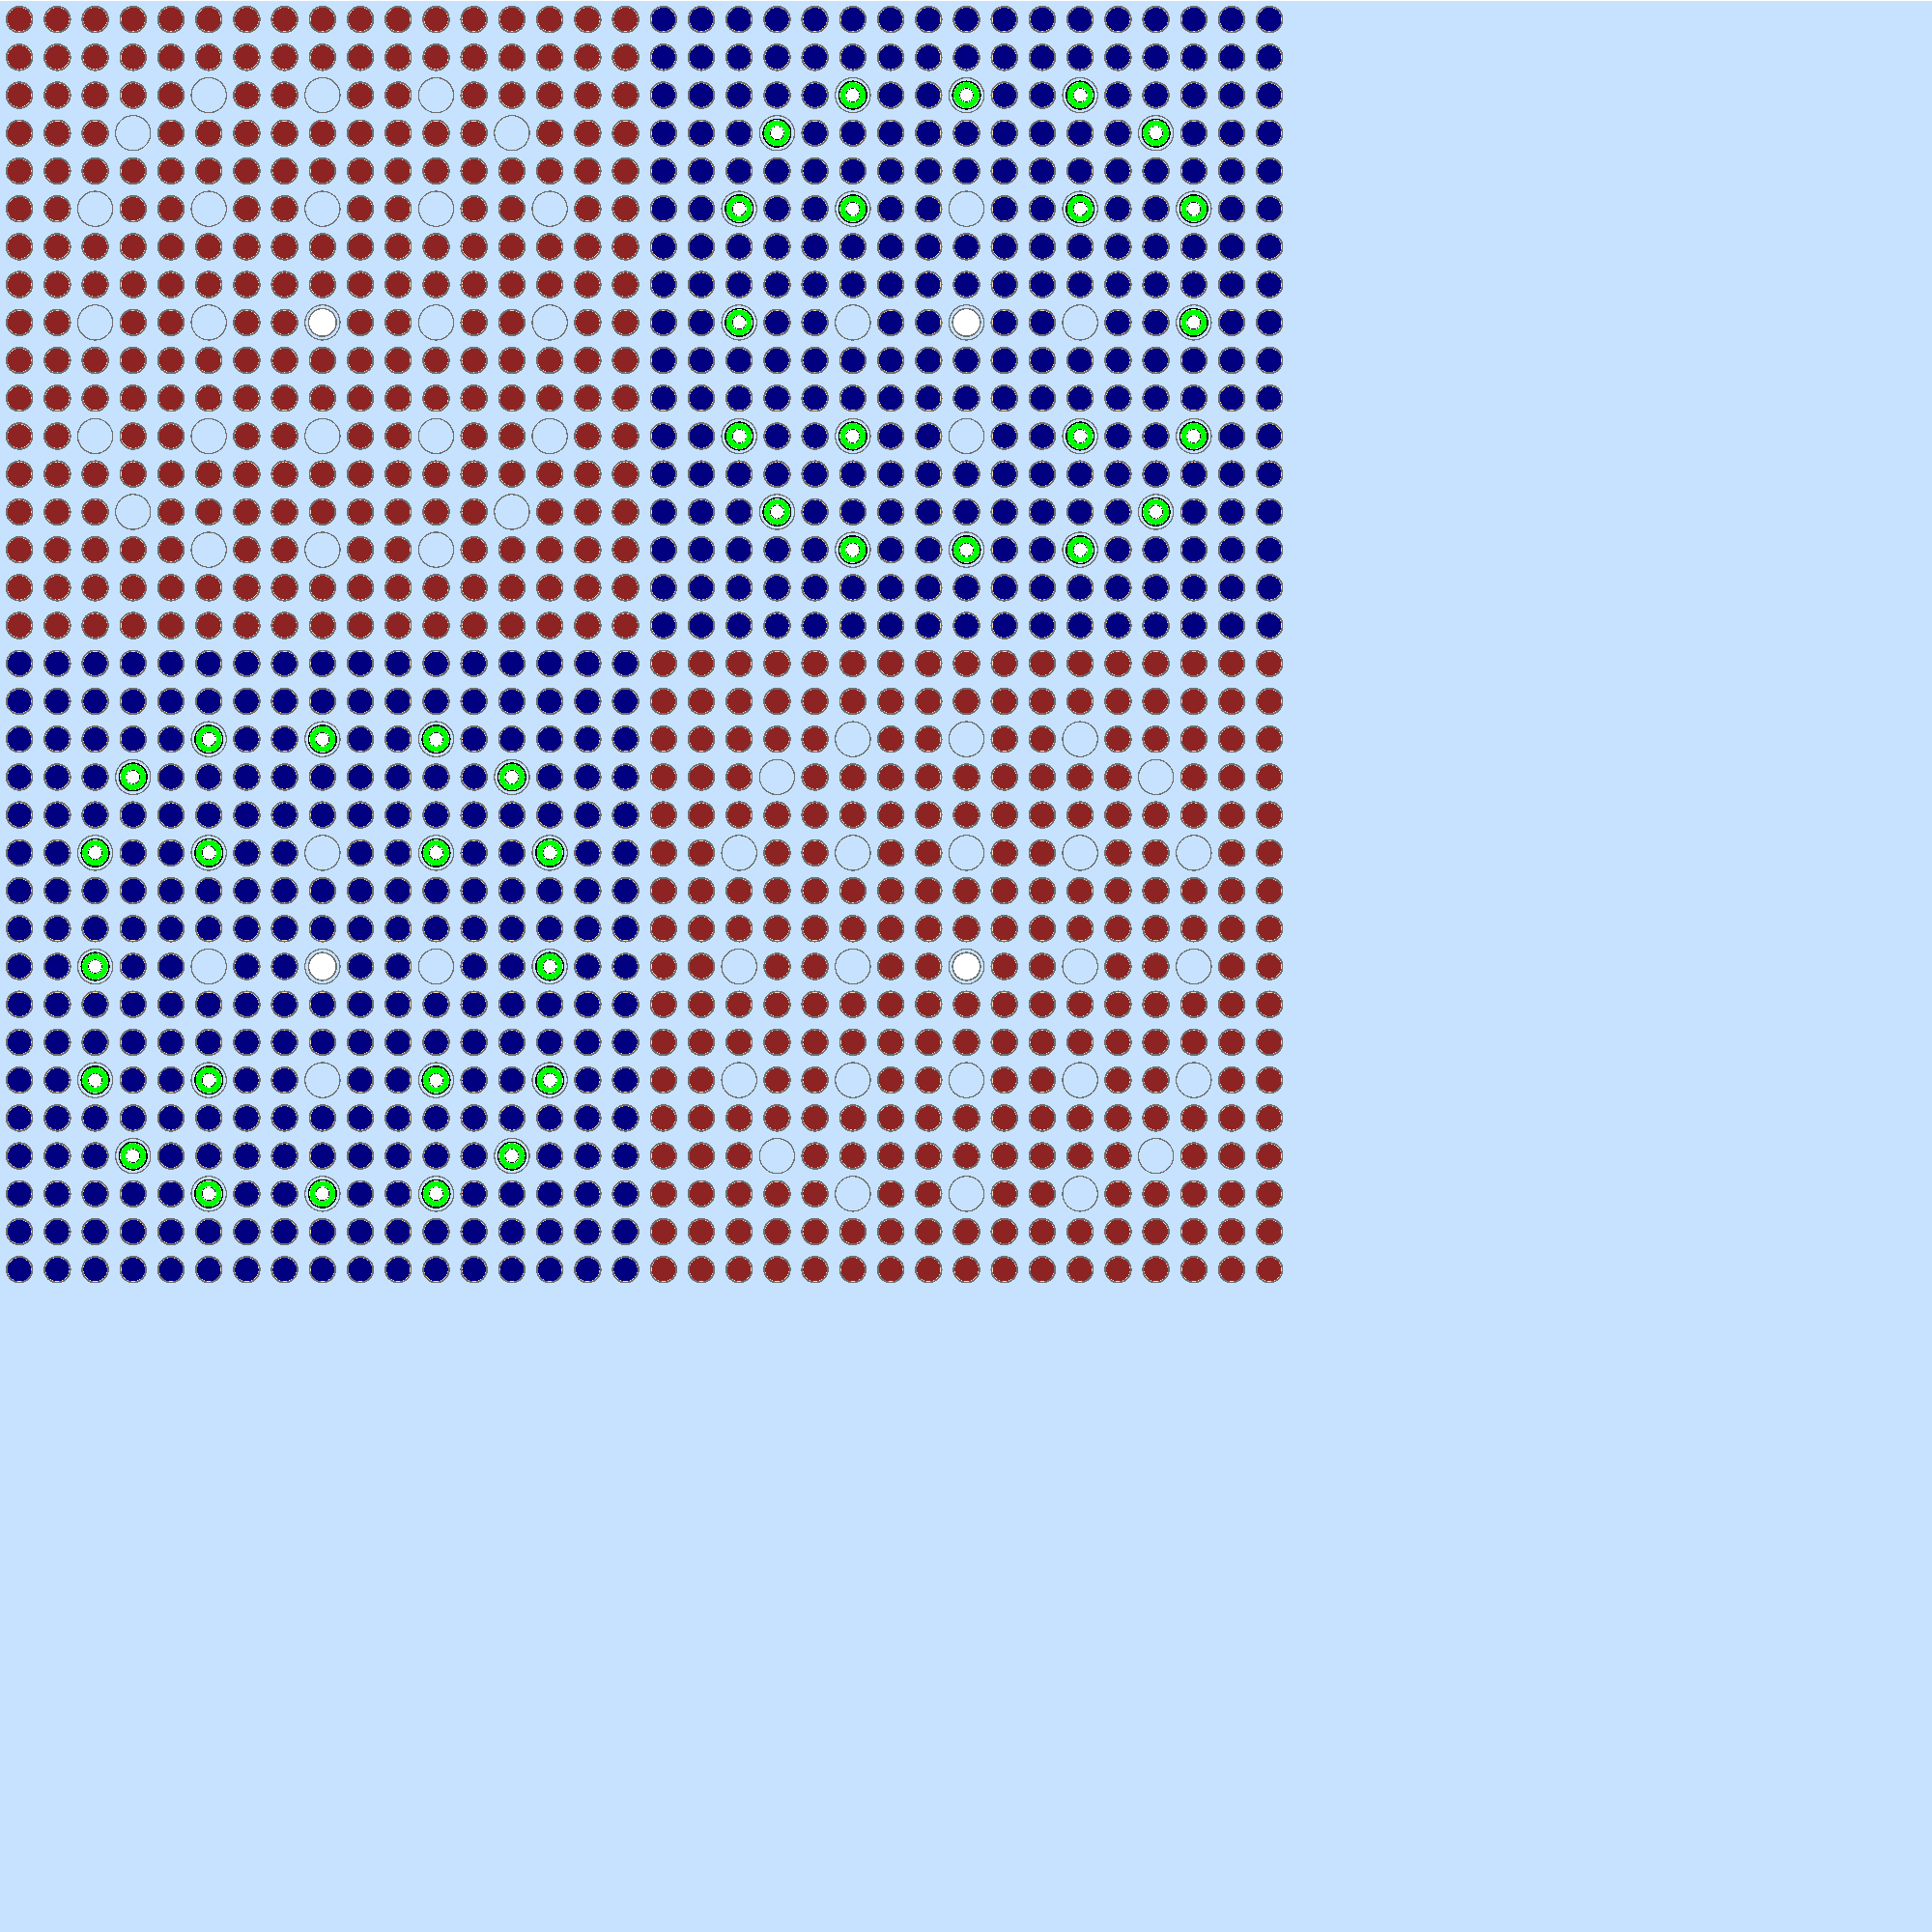
\includegraphics[width=0.8\linewidth]{figures/colorset/geometry}
  \caption{}
  \label{fig:benchmarks-colorset}
\end{subfigure}
\caption{The assembly (a) and colorset (b) benchmark geometries.}
\label{fig:benchmarks-materials}
\end{figure}

\begin{figure}[h!]
\centering
\begin{subfigure}{0.42\textwidth}
  \centering
  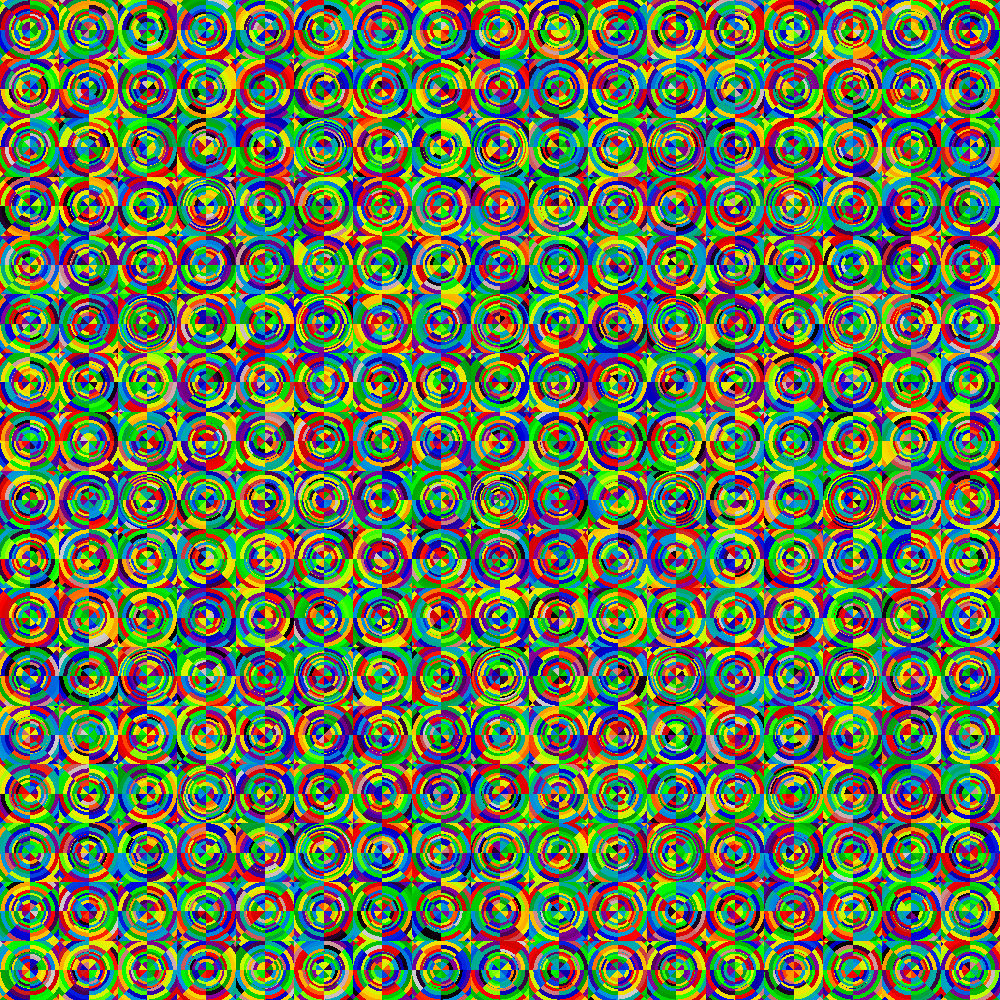
\includegraphics[width=0.8\linewidth]{figures/assembly/fsrs}
  \caption{}
  \label{fig:benchmarks-assm-fsrs}
\end{subfigure}%
\begin{subfigure}{0.42\textwidth}
  \centering
  
\includegraphics[width=0.8\linewidth]{figures/colorset/fsrs}
  \caption{}
  \label{fig:benchmarks-colorset-fsrs}
\end{subfigure}
\caption{OpenMOC flat source regions for the assembly (a) and colorset (b) benchmarks.}
\label{fig:benchmarks-fsrs}
\end{figure}

Flat source region spatial discretization meshes were applied to both benchmarks for the OpenMOC simulations as shown in \autoref{fig:benchmarks-fsrs}. The UO$_2$ fuel was subdivided into five equal volume radial rings, while ten radial rings were employed in the water-filled CRGTs and instrument tubes. The borosilicate glass and borated water material zones filling the BPs were each discretized into five equal volume radial rings. Five equally spaced rings were used in the moderator zones surrounding each pin. Eight equal angle subdivisions were used in all pin cell material zones. The 13.85824 cm of water reflector nearest the fuel assemblies in the colorset benchmark was discretized in a 0.125984 cm $\times$ 0.125984 cm rectilinear mesh, equivalent to a 10$\times$10 mesh in each pin. The 7.55904 cm of reflector furthest from the fuel assemblies was discretized in a 1.25984 cm $\times$ 1.25984 cm pin-wise mesh.

A series of OpenMC simulations was used to calculate reference eigenvalues, pin-wise fission rates, and pin-wise U-238 capture rates for both benchmarks. The reference solutions were computed with 100 inactive and 900 active batches of 10$^7$ particle histories per batch. The OpenMC ``combined'' eigenvalue estimator is reported along with the associated 1-sigma uncertainty of one pcm for both benchmarks in \autoref{tab:keff-reference}.

\begin{table}[h!]
  \centering
  \caption{Reference OpenMC eigenvalues for each benchmark.}
  \label{tab:keff-reference} 
  \begin{tabular}{c c}
  \toprule
  {\bf Assembly} &
  {\bf Colorset} \\
  \midrule
  0.99326 $\pm$ 0.00001 & 0.94574 $\pm$ 0.00001 \\
  \bottomrule
\end{tabular}
\end{table}

The reference energy-integrated fission and U-238 capture rate spatial distributions were computed using rectilinear, pin-wise tally meshes in OpenMC and are shown in \autoref{fig:fiss-capt-rates}. The reaction rates were normalized to the mean of all non-zero reaction rates. The rates in the instrument tubes, CRGTs and BPs are all zero and are shaded in white. The 1-sigma uncertainties are less than 0.08\% in each pin for both benchmarks.

\begin{figure*}[h!]
\centering
\begin{subfigure}{0.45\textwidth}
  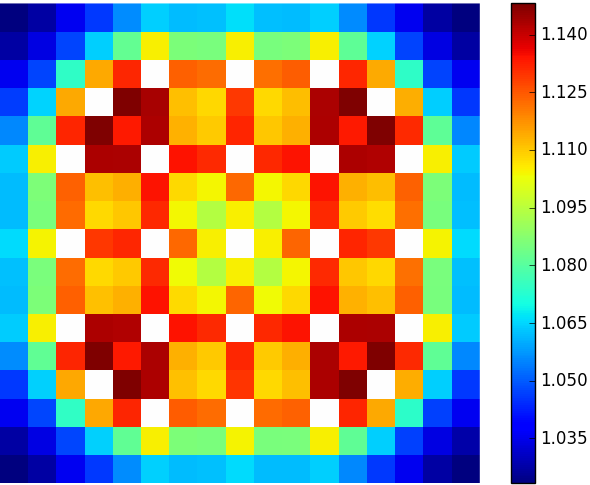
\includegraphics[width=\linewidth]{figures/assembly/fission-rates}
  \caption{}
  \label{fig:fiss-assm}
\end{subfigure}%
\begin{subfigure}{0.45\textwidth}
  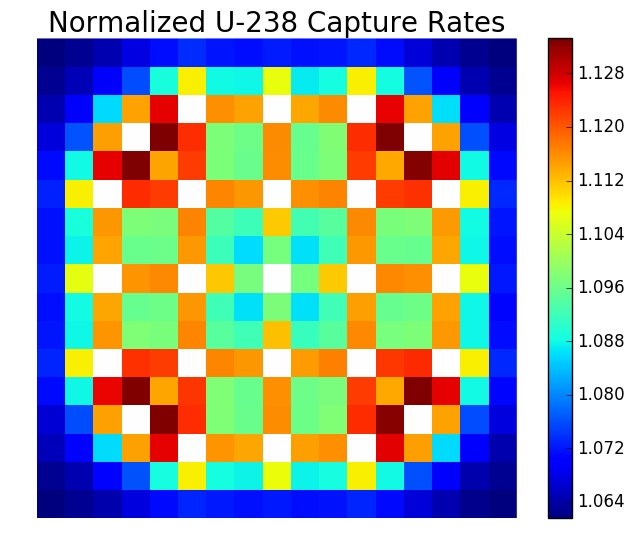
\includegraphics[width=\linewidth]{figures/assembly/capture-rates}
  \caption{}
  \label{fig:capt-assm}
\end{subfigure}
\begin{subfigure}{0.45\textwidth}
  \centering
  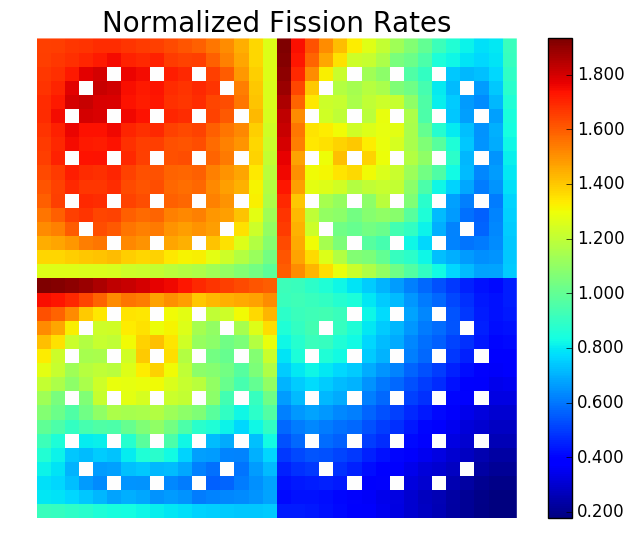
\includegraphics[width=\linewidth]{figures/colorset/fission-rates}
  \caption{}
  \label{fig:fiss-colorset}
\end{subfigure}%
\begin{subfigure}{0.45\textwidth}
  \centering
  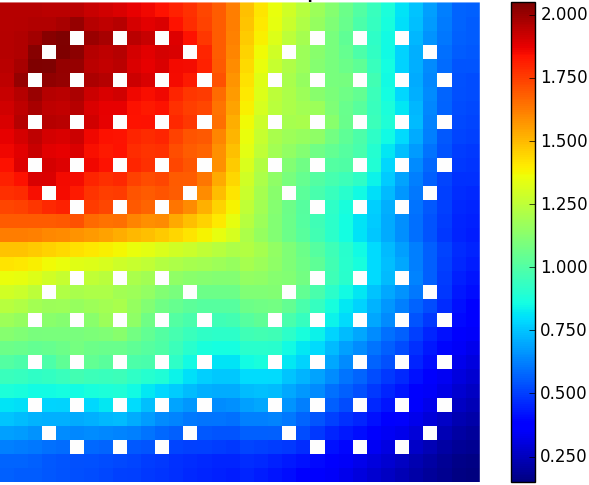
\includegraphics[width=\linewidth]{figures/colorset/capture-rates}
  \caption{}
  \label{fig:capt-colorset}
\end{subfigure}
\caption{Reference OpenMC fission and U-238 capture rates for the assembly (a) -- (b) and colorset (c) -- (d) benchmarks.}
\label{fig:benchmark-rxn-rates}
\end{figure*}